\chapter{Your First Pieces}
\label{ch:first-pieces}
\chapterline

You now know where the notes are, how scales and chords are built, how to count rhythm and how to read the staff. This chapter puts them together in real music.

There are three pieces, learned in four steps. Each step adds one new thing to the last:
\begin{itemize}
  \item \emph{Ode to Joy}, right hand: five fingers on five keys, one note per beat.
  \item \emph{Ode to Joy} with the left hand: first single bass notes, then the chords from Chapters~\ref{ch:chords-by-shape} and~\ref{ch:inversions-and-voice-leading}.
  \item \emph{Amazing Grace}: 3/4 time, a note before the first bar, a key signature and a small hand move.
  \item Four chords that fit hundreds of pop songs: an accompaniment with no melody at all.
\end{itemize}
Both melodies are old enough to be free for anyone to play.

Each piece is written three ways: as letters with finger numbers, on the staff, and as sound. Use whichever helps most, and let the others check your work.

\section{Getting ready: the C position}

Most first pieces use one hand position, so your fingers never have to search. In the C position from Chapter~\ref{ch:keyboard-geometry}, each finger of the right hand rests on one white key, starting from middle C: thumb (finger 1) on C4, then D4, E4, F4, and little finger (finger 5) on G4 \listen{C4 D4 E4 F4 G4:2}.

The left hand mirrors this, an octave lower. Little finger (5) on C3, then 4 on D3, 3 on E3, 2 on F3, and thumb (1) on G3 \listen{C3 D3 E3 F3 G3:2}. Figure~\ref{fig:c-position} shows both hands.

\begin{figure}[htbp]
\centering
\begin{tikzpicture}
\filldraw[fill=sourceblue!22, draw=black!65, line width=0.5pt] (0,0) rectangle (0.62,2.6);
\filldraw[fill=sourceblue!22, draw=black!65, line width=0.5pt] (0.62,0) rectangle (1.24,2.6);
\filldraw[fill=sourceblue!22, draw=black!65, line width=0.5pt] (1.24,0) rectangle (1.86,2.6);
\filldraw[fill=sourceblue!22, draw=black!65, line width=0.5pt] (1.86,0) rectangle (2.48,2.6);
\filldraw[fill=sourceblue!22, draw=black!65, line width=0.5pt] (2.48,0) rectangle (3.1,2.6);
\filldraw[fill=white, draw=black!65, line width=0.5pt] (3.1,0) rectangle (3.72,2.6);
\filldraw[fill=white, draw=black!65, line width=0.5pt] (3.72,0) rectangle (4.34,2.6);
\filldraw[fill=sourceblue!22, draw=black!65, line width=0.5pt] (4.34,0) rectangle (4.96,2.6);
\filldraw[fill=sourceblue!22, draw=black!65, line width=0.5pt] (4.96,0) rectangle (5.58,2.6);
\filldraw[fill=sourceblue!22, draw=black!65, line width=0.5pt] (5.58,0) rectangle (6.2,2.6);
\filldraw[fill=sourceblue!22, draw=black!65, line width=0.5pt] (6.2,0) rectangle (6.82,2.6);
\filldraw[fill=sourceblue!22, draw=black!65, line width=0.5pt] (6.82,0) rectangle (7.44,2.6);
\filldraw[fill=white, draw=black!65, line width=0.5pt] (7.44,0) rectangle (8.06,2.6);
\filldraw[fill=white, draw=black!65, line width=0.5pt] (8.06,0) rectangle (8.68,2.6);
\filldraw[fill=black!85, draw=black, line width=0.4pt] (0.49,0.988) rectangle (0.75,2.6);
\filldraw[fill=black!85, draw=black, line width=0.4pt] (1.11,0.988) rectangle (1.37,2.6);
\filldraw[fill=black!85, draw=black, line width=0.4pt] (2.35,0.988) rectangle (2.61,2.6);
\filldraw[fill=black!85, draw=black, line width=0.4pt] (2.97,0.988) rectangle (3.23,2.6);
\filldraw[fill=black!85, draw=black, line width=0.4pt] (3.59,0.988) rectangle (3.85,2.6);
\filldraw[fill=black!85, draw=black, line width=0.4pt] (4.83,0.988) rectangle (5.09,2.6);
\filldraw[fill=black!85, draw=black, line width=0.4pt] (5.45,0.988) rectangle (5.71,2.6);
\filldraw[fill=black!85, draw=black, line width=0.4pt] (6.69,0.988) rectangle (6.95,2.6);
\filldraw[fill=black!85, draw=black, line width=0.4pt] (7.31,0.988) rectangle (7.57,2.6);
\filldraw[fill=black!85, draw=black, line width=0.4pt] (7.93,0.988) rectangle (8.19,2.6);
\node[font=\small] at (0.31,0.3) {5};
\node[font=\small] at (0.93,0.3) {4};
\node[font=\small] at (1.55,0.3) {3};
\node[font=\small] at (2.17,0.3) {2};
\node[font=\small] at (2.79,0.3) {1};
\node[font=\small] at (4.65,0.3) {1};
\node[font=\small] at (5.27,0.3) {2};
\node[font=\small] at (5.89,0.3) {3};
\node[font=\small] at (6.51,0.3) {4};
\node[font=\small] at (7.13,0.3) {5};
\node[font=\small] at (0.31,-0.35) {C3};
\node[font=\small] at (2.79,-0.35) {G3};
\node[font=\small] at (4.65,-0.35) {C4};
\node[font=\small] at (7.13,-0.35) {G4};
\node[font=\small] at (1.55,3) {left hand};
\node[font=\small] at (5.89,3) {right hand};
\end{tikzpicture}
\caption{The C position. The numbers are the fingers that rest on each key: thumbs are 1, little fingers are 5.}
\label{fig:c-position}
\end{figure}

Sit so your forearms are about level with the keys. Curve your fingers gently, as if holding a ball, and play with the fleshy tips. Keep your shoulders loose.

\begin{tryitbox}
Place your right hand in C position. Play C, D, E, F, G and back down, saying the finger numbers out loud: 1, 2, 3, 4, 5, 4, 3, 2, 1 \listen{C4 D4 E4 F4 G4 F4 E4 D4 C4:2}. Do the same with the left hand: 5, 4, 3, 2, 1, 2, 3, 4, 5 \listen{C3 D3 E3 F3 G3 F3 E3 D3 C3:2}.
\end{tryitbox}

\section{Ode to Joy: the right hand}

Beethoven wrote this tune for the last movement of his Ninth Symphony, in 1824. It moves mostly by steps, so the whole tune fits under a hand in C position: the five keys you have been playing are all it needs. Its time signature is 4/4, and almost every note is a quarter note: one note per beat.

The tune has two phrases. A \textbf{phrase} is a musical sentence, a few bars long, that ends with a feeling of a pause. Here is the first one, bar by bar:

\begin{center}
\begin{tabular}{lllll}
\toprule
 & bar 1 & bar 2 & bar 3 & bar 4 \\
\midrule
notes & E E F G & G F E D & C C D E & E. D D \\
fingers & 3 3 4 5 & 5 4 3 2 & 1 1 2 3 & 3 2 2 \\
\bottomrule
\end{tabular}
\end{center}

Bars 1 to 3 are four quarter notes each. Bar 4 is the rhythm from Chapter~\ref{ch:beats-timing-and-reading}: a dotted quarter (the ``E.''), an eighth note, and a half note. Count ``1 and 2 and 3 and 4 and'': E on 1, the first D on the ``and'' after 2, and the last D on 3, held to the end of the bar.

Listen to the first phrase \listen{@100 E4 E4 F4 G4 G4 F4 E4 D4 C4 C4 D4 E4 E4:1.5 D4:0.5 D4:2}. It ends on D, which sounds a little unfinished, like a question.

The second phrase starts the same way. Only the last bar changes, and it ends on C, which sounds like an answer:

\begin{center}
\begin{tabular}{lllll}
\toprule
 & bar 5 & bar 6 & bar 7 & bar 8 \\
\midrule
notes & E E F G & G F E D & C C D E & D. C C \\
fingers & 3 3 4 5 & 5 4 3 2 & 1 1 2 3 & 2 1 1 \\
\bottomrule
\end{tabular}
\end{center}

Listen to the second phrase \listen{@100 E4 E4 F4 G4 G4 F4 E4 D4 C4 C4 D4 E4 D4:1.5 C4:0.5 C4:2}, then to both phrases together \listen{@100 E4 E4 F4 G4 G4 F4 E4 D4 C4 C4 D4 E4 E4:1.5 D4:0.5 D4:2 E4 E4 F4 G4 G4 F4 E4 D4 C4 C4 D4 E4 D4:1.5 C4:0.5 C4:2}.

Figure~\ref{fig:ode} shows the same melody on the treble staff, with finger numbers above the notes and letters below. Look at how the noteheads climb and fall one step at a time, line to space to line, and how each step up the staff is one finger further along.

\begin{figure}[htbp]
\centering
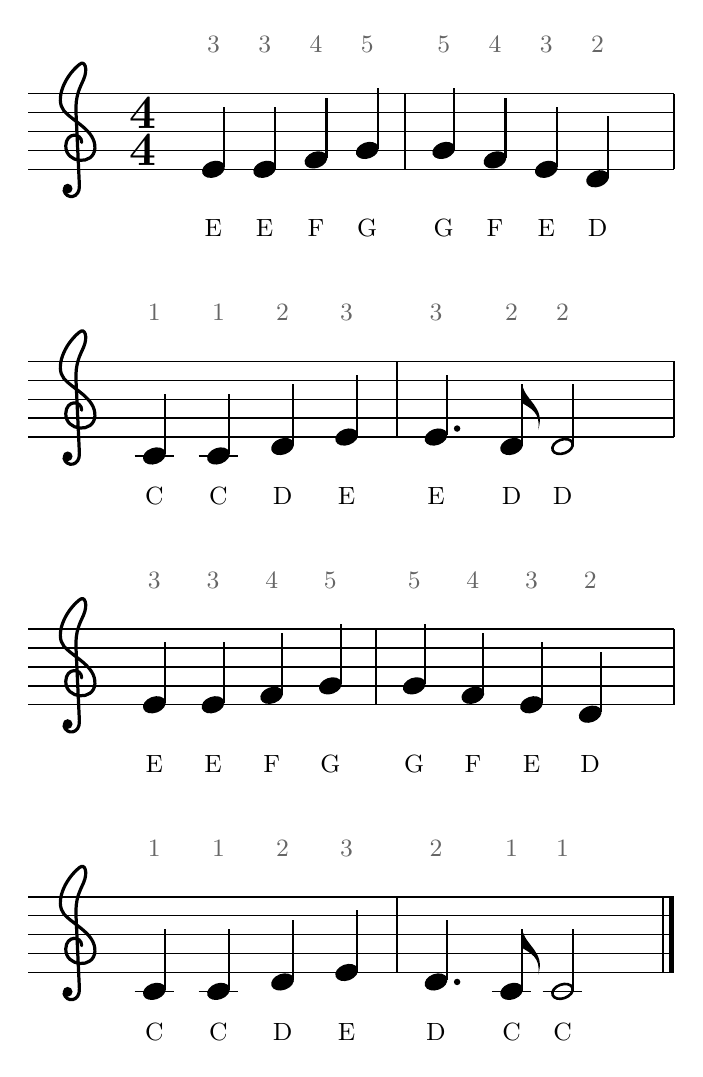
\begin{tikzpicture}
\draw[line width=0.5pt] (0,0) -- (8.2,0);
\draw[line width=0.5pt] (0,0.24) -- (8.2,0.24);
\draw[line width=0.5pt] (0,0.48) -- (8.2,0.48);
\draw[line width=0.5pt] (0,0.72) -- (8.2,0.72);
\draw[line width=0.5pt] (0,0.96) -- (8.2,0.96);
\draw[black, line width=1.161pt, line cap=round] (0.677,0.341) .. controls (0.677,0.468) and (0.48,0.475) .. (0.475,0.3) .. controls (0.468,0.072) and (0.835,0.043) .. (0.845,0.269) .. controls (0.854,0.492) and (0.576,0.6) .. (0.451,0.744) .. controls (0.336,0.888) and (0.456,1.176) .. (0.648,1.332) .. controls (0.72,1.392) and (0.758,1.272) .. (0.701,1.14) .. controls (0.653,1.032) and (0.595,0.936) .. (0.605,0.72) -- (0.648,-0.204) .. controls (0.658,-0.372) and (0.48,-0.389) .. (0.451,-0.264);
\fill[black] (0.499,-0.245) circle (0.062);
\node[font=\bfseries\LARGE, inner sep=0] at (1.45,0.72) {4};
\node[font=\bfseries\LARGE, inner sep=0] at (1.45,0.24) {4};
\fill[black, rotate around={20:(2.35,0)}] (2.35,0) ellipse (0.149 and 0.103);
\draw[black, line width=0.75pt] (2.484,0.024) -- (2.484,0.792);
\node[font=\small] at (2.35,-0.75) {E};
\node[font=\small, text=black!60] at (2.35,1.58) {3};
\fill[black, rotate around={20:(3.001,0)}] (3.001,0) ellipse (0.149 and 0.103);
\draw[black, line width=0.75pt] (3.135,0.024) -- (3.135,0.792);
\node[font=\small] at (3.001,-0.75) {E};
\node[font=\small, text=black!60] at (3.001,1.58) {3};
\fill[black, rotate around={20:(3.652,0.12)}] (3.652,0.12) ellipse (0.149 and 0.103);
\draw[black, line width=0.75pt] (3.786,0.144) -- (3.786,0.912);
\node[font=\small] at (3.652,-0.75) {F};
\node[font=\small, text=black!60] at (3.652,1.58) {4};
\fill[black, rotate around={20:(4.304,0.24)}] (4.304,0.24) ellipse (0.149 and 0.103);
\draw[black, line width=0.75pt] (4.438,0.264) -- (4.438,1.032);
\node[font=\small] at (4.304,-0.75) {G};
\node[font=\small, text=black!60] at (4.304,1.58) {5};
\draw[line width=0.7pt] (4.785,0) -- (4.785,0.96);
\fill[black, rotate around={20:(5.275,0.24)}] (5.275,0.24) ellipse (0.149 and 0.103);
\draw[black, line width=0.75pt] (5.409,0.264) -- (5.409,1.032);
\node[font=\small] at (5.275,-0.75) {G};
\node[font=\small, text=black!60] at (5.275,1.58) {5};
\fill[black, rotate around={20:(5.926,0.12)}] (5.926,0.12) ellipse (0.149 and 0.103);
\draw[black, line width=0.75pt] (6.06,0.144) -- (6.06,0.912);
\node[font=\small] at (5.926,-0.75) {F};
\node[font=\small, text=black!60] at (5.926,1.58) {4};
\fill[black, rotate around={20:(6.578,0)}] (6.578,0) ellipse (0.149 and 0.103);
\draw[black, line width=0.75pt] (6.711,0.024) -- (6.711,0.792);
\node[font=\small] at (6.578,-0.75) {E};
\node[font=\small, text=black!60] at (6.578,1.58) {3};
\fill[black, rotate around={20:(7.229,-0.12)}] (7.229,-0.12) ellipse (0.149 and 0.103);
\draw[black, line width=0.75pt] (7.363,-0.096) -- (7.363,0.672);
\node[font=\small] at (7.229,-0.75) {D};
\node[font=\small, text=black!60] at (7.229,1.58) {2};
\draw[line width=0.7pt] (8.2,0) -- (8.2,0.96);
\draw[line width=0.5pt] (0,-3.4) -- (8.2,-3.4);
\draw[line width=0.5pt] (0,-3.16) -- (8.2,-3.16);
\draw[line width=0.5pt] (0,-2.92) -- (8.2,-2.92);
\draw[line width=0.5pt] (0,-2.68) -- (8.2,-2.68);
\draw[line width=0.5pt] (0,-2.44) -- (8.2,-2.44);
\draw[black, line width=1.161pt, line cap=round] (0.677,-3.059) .. controls (0.677,-2.932) and (0.48,-2.925) .. (0.475,-3.1) .. controls (0.468,-3.328) and (0.835,-3.357) .. (0.845,-3.131) .. controls (0.854,-2.908) and (0.576,-2.8) .. (0.451,-2.656) .. controls (0.336,-2.512) and (0.456,-2.224) .. (0.648,-2.068) .. controls (0.72,-2.008) and (0.758,-2.128) .. (0.701,-2.26) .. controls (0.653,-2.368) and (0.595,-2.464) .. (0.605,-2.68) -- (0.648,-3.604) .. controls (0.658,-3.772) and (0.48,-3.789) .. (0.451,-3.664);
\fill[black] (0.499,-3.645) circle (0.062);
\draw[black, line width=0.6pt] (1.348,-3.64) -- (1.852,-3.64);
\fill[black, rotate around={20:(1.6,-3.64)}] (1.6,-3.64) ellipse (0.149 and 0.103);
\draw[black, line width=0.75pt] (1.734,-3.616) -- (1.734,-2.848);
\node[font=\small] at (1.6,-4.15) {C};
\node[font=\small, text=black!60] at (1.6,-1.82) {1};
\draw[black, line width=0.6pt] (2.162,-3.64) -- (2.666,-3.64);
\fill[black, rotate around={20:(2.414,-3.64)}] (2.414,-3.64) ellipse (0.149 and 0.103);
\draw[black, line width=0.75pt] (2.548,-3.616) -- (2.548,-2.848);
\node[font=\small] at (2.414,-4.15) {C};
\node[font=\small, text=black!60] at (2.414,-1.82) {1};
\fill[black, rotate around={20:(3.228,-3.52)}] (3.228,-3.52) ellipse (0.149 and 0.103);
\draw[black, line width=0.75pt] (3.362,-3.496) -- (3.362,-2.728);
\node[font=\small] at (3.228,-4.15) {D};
\node[font=\small, text=black!60] at (3.228,-1.82) {2};
\fill[black, rotate around={20:(4.042,-3.4)}] (4.042,-3.4) ellipse (0.149 and 0.103);
\draw[black, line width=0.75pt] (4.176,-3.376) -- (4.176,-2.608);
\node[font=\small] at (4.042,-4.15) {E};
\node[font=\small, text=black!60] at (4.042,-1.82) {3};
\draw[line width=0.7pt] (4.687,-3.4) -- (4.687,-2.44);
\fill[black, rotate around={20:(5.177,-3.4)}] (5.177,-3.4) ellipse (0.149 and 0.103);
\draw[black, line width=0.75pt] (5.311,-3.376) -- (5.311,-2.608);
\fill[black] (5.445,-3.292) circle (0.041);
\node[font=\small] at (5.177,-4.15) {E};
\node[font=\small, text=black!60] at (5.177,-1.82) {3};
\fill[black, rotate around={20:(6.137,-3.52)}] (6.137,-3.52) ellipse (0.149 and 0.103);
\draw[black, line width=0.75pt] (6.271,-3.496) -- (6.271,-2.728);
\fill[black] (6.271,-2.728) .. controls (6.307,-2.944) and (6.571,-3.016) .. (6.475,-3.304) .. controls (6.511,-3.088) and (6.367,-3.028) .. (6.271,-2.968) -- cycle;
\node[font=\small] at (6.137,-4.15) {D};
\node[font=\small, text=black!60] at (6.137,-1.82) {2};
\draw[black, line width=0.95pt, rotate around={20:(6.784,-3.52)}] (6.784,-3.52) ellipse (0.134 and 0.088);
\draw[black, line width=0.75pt] (6.918,-3.496) -- (6.918,-2.728);
\node[font=\small] at (6.784,-4.15) {D};
\node[font=\small, text=black!60] at (6.784,-1.82) {2};
\draw[line width=0.7pt] (8.2,-3.4) -- (8.2,-2.44);
\draw[line width=0.5pt] (0,-6.8) -- (8.2,-6.8);
\draw[line width=0.5pt] (0,-6.56) -- (8.2,-6.56);
\draw[line width=0.5pt] (0,-6.32) -- (8.2,-6.32);
\draw[line width=0.5pt] (0,-6.08) -- (8.2,-6.08);
\draw[line width=0.5pt] (0,-5.84) -- (8.2,-5.84);
\draw[black, line width=1.161pt, line cap=round] (0.677,-6.459) .. controls (0.677,-6.332) and (0.48,-6.325) .. (0.475,-6.5) .. controls (0.468,-6.728) and (0.835,-6.757) .. (0.845,-6.531) .. controls (0.854,-6.308) and (0.576,-6.2) .. (0.451,-6.056) .. controls (0.336,-5.912) and (0.456,-5.624) .. (0.648,-5.468) .. controls (0.72,-5.408) and (0.758,-5.528) .. (0.701,-5.66) .. controls (0.653,-5.768) and (0.595,-5.864) .. (0.605,-6.08) -- (0.648,-7.004) .. controls (0.658,-7.172) and (0.48,-7.189) .. (0.451,-7.064);
\fill[black] (0.499,-7.045) circle (0.062);
\fill[black, rotate around={20:(1.6,-6.8)}] (1.6,-6.8) ellipse (0.149 and 0.103);
\draw[black, line width=0.75pt] (1.734,-6.776) -- (1.734,-6.008);
\node[font=\small] at (1.6,-7.55) {E};
\node[font=\small, text=black!60] at (1.6,-5.22) {3};
\fill[black, rotate around={20:(2.345,-6.8)}] (2.345,-6.8) ellipse (0.149 and 0.103);
\draw[black, line width=0.75pt] (2.479,-6.776) -- (2.479,-6.008);
\node[font=\small] at (2.345,-7.55) {E};
\node[font=\small, text=black!60] at (2.345,-5.22) {3};
\fill[black, rotate around={20:(3.09,-6.68)}] (3.09,-6.68) ellipse (0.149 and 0.103);
\draw[black, line width=0.75pt] (3.224,-6.656) -- (3.224,-5.888);
\node[font=\small] at (3.09,-7.55) {F};
\node[font=\small, text=black!60] at (3.09,-5.22) {4};
\fill[black, rotate around={20:(3.835,-6.56)}] (3.835,-6.56) ellipse (0.149 and 0.103);
\draw[black, line width=0.75pt] (3.969,-6.536) -- (3.969,-5.768);
\node[font=\small] at (3.835,-7.55) {G};
\node[font=\small, text=black!60] at (3.835,-5.22) {5};
\draw[line width=0.7pt] (4.41,-6.8) -- (4.41,-5.84);
\fill[black, rotate around={20:(4.9,-6.56)}] (4.9,-6.56) ellipse (0.149 and 0.103);
\draw[black, line width=0.75pt] (5.034,-6.536) -- (5.034,-5.768);
\node[font=\small] at (4.9,-7.55) {G};
\node[font=\small, text=black!60] at (4.9,-5.22) {5};
\fill[black, rotate around={20:(5.645,-6.68)}] (5.645,-6.68) ellipse (0.149 and 0.103);
\draw[black, line width=0.75pt] (5.779,-6.656) -- (5.779,-5.888);
\node[font=\small] at (5.645,-7.55) {F};
\node[font=\small, text=black!60] at (5.645,-5.22) {4};
\fill[black, rotate around={20:(6.39,-6.8)}] (6.39,-6.8) ellipse (0.149 and 0.103);
\draw[black, line width=0.75pt] (6.524,-6.776) -- (6.524,-6.008);
\node[font=\small] at (6.39,-7.55) {E};
\node[font=\small, text=black!60] at (6.39,-5.22) {3};
\fill[black, rotate around={20:(7.135,-6.92)}] (7.135,-6.92) ellipse (0.149 and 0.103);
\draw[black, line width=0.75pt] (7.269,-6.896) -- (7.269,-6.128);
\node[font=\small] at (7.135,-7.55) {D};
\node[font=\small, text=black!60] at (7.135,-5.22) {2};
\draw[line width=0.7pt] (8.2,-6.8) -- (8.2,-5.84);
\draw[line width=0.5pt] (0,-10.2) -- (8.2,-10.2);
\draw[line width=0.5pt] (0,-9.96) -- (8.2,-9.96);
\draw[line width=0.5pt] (0,-9.72) -- (8.2,-9.72);
\draw[line width=0.5pt] (0,-9.48) -- (8.2,-9.48);
\draw[line width=0.5pt] (0,-9.24) -- (8.2,-9.24);
\draw[black, line width=1.161pt, line cap=round] (0.677,-9.859) .. controls (0.677,-9.732) and (0.48,-9.725) .. (0.475,-9.9) .. controls (0.468,-10.128) and (0.835,-10.157) .. (0.845,-9.931) .. controls (0.854,-9.708) and (0.576,-9.6) .. (0.451,-9.456) .. controls (0.336,-9.312) and (0.456,-9.024) .. (0.648,-8.868) .. controls (0.72,-8.808) and (0.758,-8.928) .. (0.701,-9.06) .. controls (0.653,-9.168) and (0.595,-9.264) .. (0.605,-9.48) -- (0.648,-10.404) .. controls (0.658,-10.572) and (0.48,-10.589) .. (0.451,-10.464);
\fill[black] (0.499,-10.445) circle (0.062);
\draw[black, line width=0.6pt] (1.348,-10.44) -- (1.852,-10.44);
\fill[black, rotate around={20:(1.6,-10.44)}] (1.6,-10.44) ellipse (0.149 and 0.103);
\draw[black, line width=0.75pt] (1.734,-10.416) -- (1.734,-9.648);
\node[font=\small] at (1.6,-10.95) {C};
\node[font=\small, text=black!60] at (1.6,-8.62) {1};
\draw[black, line width=0.6pt] (2.162,-10.44) -- (2.666,-10.44);
\fill[black, rotate around={20:(2.414,-10.44)}] (2.414,-10.44) ellipse (0.149 and 0.103);
\draw[black, line width=0.75pt] (2.548,-10.416) -- (2.548,-9.648);
\node[font=\small] at (2.414,-10.95) {C};
\node[font=\small, text=black!60] at (2.414,-8.62) {1};
\fill[black, rotate around={20:(3.228,-10.32)}] (3.228,-10.32) ellipse (0.149 and 0.103);
\draw[black, line width=0.75pt] (3.362,-10.296) -- (3.362,-9.528);
\node[font=\small] at (3.228,-10.95) {D};
\node[font=\small, text=black!60] at (3.228,-8.62) {2};
\fill[black, rotate around={20:(4.042,-10.2)}] (4.042,-10.2) ellipse (0.149 and 0.103);
\draw[black, line width=0.75pt] (4.176,-10.176) -- (4.176,-9.408);
\node[font=\small] at (4.042,-10.95) {E};
\node[font=\small, text=black!60] at (4.042,-8.62) {3};
\draw[line width=0.7pt] (4.687,-10.2) -- (4.687,-9.24);
\fill[black, rotate around={20:(5.177,-10.32)}] (5.177,-10.32) ellipse (0.149 and 0.103);
\draw[black, line width=0.75pt] (5.311,-10.296) -- (5.311,-9.528);
\fill[black] (5.445,-10.32) circle (0.041);
\node[font=\small] at (5.177,-10.95) {D};
\node[font=\small, text=black!60] at (5.177,-8.62) {2};
\draw[black, line width=0.6pt] (5.885,-10.44) -- (6.389,-10.44);
\fill[black, rotate around={20:(6.137,-10.44)}] (6.137,-10.44) ellipse (0.149 and 0.103);
\draw[black, line width=0.75pt] (6.271,-10.416) -- (6.271,-9.648);
\fill[black] (6.271,-9.648) .. controls (6.307,-9.864) and (6.571,-9.936) .. (6.475,-10.224) .. controls (6.511,-10.008) and (6.367,-9.948) .. (6.271,-9.888) -- cycle;
\node[font=\small] at (6.137,-10.95) {C};
\node[font=\small, text=black!60] at (6.137,-8.62) {1};
\draw[black, line width=0.6pt] (6.532,-10.44) -- (7.036,-10.44);
\draw[black, line width=0.95pt, rotate around={20:(6.784,-10.44)}] (6.784,-10.44) ellipse (0.134 and 0.088);
\draw[black, line width=0.75pt] (6.918,-10.416) -- (6.918,-9.648);
\node[font=\small] at (6.784,-10.95) {C};
\node[font=\small, text=black!60] at (6.784,-8.62) {1};
\draw[line width=0.6pt] (8.06,-10.2) -- (8.06,-9.24);
\fill (8.13,-10.2) rectangle (8.2,-9.24);
\end{tikzpicture}
\caption{Ode to Joy, both phrases, in C position. Finger numbers are above the staff and note names below.}
\label{fig:ode}
\end{figure}

\begin{tryitbox}
Play the first phrase slowly, at about half the speed of the recording, counting out loud. If you play a wrong note, keep going to the end. Then play it three more times. When it feels steady, learn the second phrase, which only changes in the last bar.
\end{tryitbox}

\section{Ode to Joy: adding the left hand}

Now give the melody a floor to stand on. We add the left hand in two stages: first single bass notes, then full chords.

\subsection*{Stage 1: bass notes}

Put your left hand in C position. You need only two keys: C3 under your little finger (5) and G3 under your thumb (1). C goes with the C major chord and G with the G major chord, the I and V chords of the key of C from Chapter~\ref{ch:chords-by-shape}.

How do you know which one fits a bar? Look at the melody. Bar 1 (E, E, F, G) leans on E and G, two notes of the C chord, so C goes under it. Bar 2 (G, F, E, D) leans on G and D, two notes of the G chord (G, B, D), so G goes under it.

Play one bass note at the start of each bar, together with the first melody note, and hold it while the right hand carries on. In the last bar of each phrase, the bass changes halfway, on beat 3:

\begin{center}
\begin{tabular}{lllllllll}
\toprule
bar & 1 & 2 & 3 & 4 & 5 & 6 & 7 & 8 \\
\midrule
left hand & C & G & C & C, then G & C & G & C & G, then C \\
\bottomrule
\end{tabular}
\end{center}

Listen to the first phrase with bass notes \listen{@100 =C3:4 E4 E4 F4 G4 =G3:4 G4 F4 E4 D4 =C3:4 C4 C4 D4 E4 =C3:2 E4:1.5 D4:0.5 =G3:2 D4:2} and the second \listen{@100 =C3:4 E4 E4 F4 G4 =G3:4 G4 F4 E4 D4 =C3:4 C4 C4 D4 E4 =G3:2 D4:1.5 C4:0.5 =C3:2 C4:2}.

Practice each hand alone first. Then put them together slowly, using the T/R/L idea from Chapter~\ref{ch:beats-timing-and-reading}: on the first beat of each bar both hands play (T), and on the other beats only the right hand plays (R). The one exception is beat 3 of each phrase's last bar, where the bass changes: that beat is T as well.

\subsection*{Stage 2: chords}

When the bass notes feel easy, replace them with three-note chords. The C chord is C3--E3--G3, with fingers 5, 3 and 1 \listen{C3+E3+G3:2}.

For the G chord, use the smooth change from Chapter~\ref{ch:inversions-and-voice-leading}. Keep your thumb on G3. Move your middle finger down one white key, from E3 to D3, and your little finger down a half step, from C3 to B2. That gives B2--D3--G3, a G chord in first inversion, with fingers 5, 3, 1 \listen{B2+D3+G3:2}. Your hand hardly moves: C chord, G chord, C chord \listen{C3+E3+G3:2 B2+D3+G3:2 C3+E3+G3:2}.

Play each chord where the table above has its bass note. Here is the first phrase with chords \listen{@100 =C3+E3+G3:4 E4 E4 F4 G4 =B2+D3+G3:4 G4 F4 E4 D4 =C3+E3+G3:4 C4 C4 D4 E4 =C3+E3+G3:2 E4:1.5 D4:0.5 =B2+D3+G3:2 D4:2} and the second \listen{@100 =C3+E3+G3:4 E4 E4 F4 G4 =B2+D3+G3:4 G4 F4 E4 D4 =C3+E3+G3:4 C4 C4 D4 E4 =B2+D3+G3:2 D4:1.5 C4:0.5 =C3+E3+G3:2 C4:2}.

\section{Amazing Grace: a song in 3/4}

\emph{Amazing Grace} is a hymn from the 1770s, sung to an American folk tune. Ode to Joy stayed in one hand position, in 4/4, with no key signature. This song changes each of those, one at a time. It is in 3/4 time, so count ``\textbf{1}, 2, 3'' with a gentle lean on each 1. Here is its first line, ``Amazing grace, how sweet the sound, that saved a wretch like me''.

\subsection*{The pickup note}

The song does not start on beat 1. Its first word, ``A-'', comes on beat 3, directly before the first full bar. A note like this, before the first bar line, is called a \textbf{pickup}. Count ``1, 2'' silently, play the pickup on ``3'', and the next note lands on the strong beat 1.

\subsection*{The right hand}

This song is in the key of G, which has one sharp, F\sh. You can see it as the key signature after the clef in Figure~\ref{fig:grace}. The first line happens not to use F at all, so you will not need a black key yet.

Place your right thumb on D4, finger 2 on E4, finger 3 on G4, finger 4 on A4 and finger 5 on B4. (Your hand skips over F\sh.) Only the last note, D5, is out of reach: lift your hand and play it with finger 5. A small move like this is normal.

\begin{center}
\begin{tabular}{llllll}
\toprule
bar & words & notes & fingers & beats & left hand \\
\midrule
pickup & A- & D & 1 & 1 & -- \\
1 & -maz-ing & G, B G & 3, 5 3 & 2, half + half & G \\
2 & grace, how & B, A & 5, 4 & 2, 1 & G \\
3 & sweet the & G, E & 3, 2 & 2, 1 & C \\
4 & sound, that & D, D & 1, 1 & 2, 1 & G \\
5 & saved a & G, B G & 3, 5 3 & 2, half + half & G \\
6 & wretch like & B, A & 5, 4 & 2, 1 & G \\
7 & me & D (high) & 5 & 3 & D \\
\bottomrule
\end{tabular}
\end{center}

``-maz-ing'' has a half note on ``maz'', then two eighth notes, B and G, on ``-ing''. The last note is a dotted half note, held for the whole bar. Listen \listen{@84 D4 G4:2 B4:0.5 G4:0.5 B4:2 A4 G4:2 E4 D4:2 D4 G4:2 B4:0.5 G4:0.5 B4:2 A4 D5:3}.

\begin{figure}[htbp]
\centering
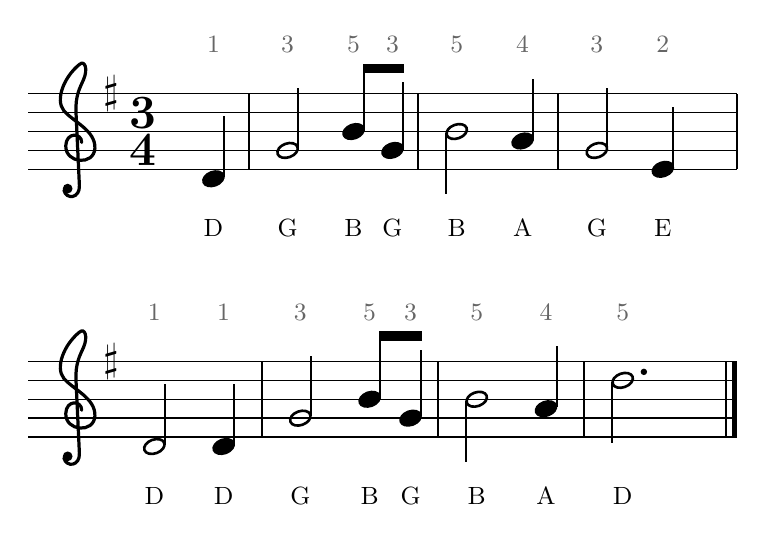
\begin{tikzpicture}
\draw[line width=0.5pt] (0,0) -- (9,0);
\draw[line width=0.5pt] (0,0.24) -- (9,0.24);
\draw[line width=0.5pt] (0,0.48) -- (9,0.48);
\draw[line width=0.5pt] (0,0.72) -- (9,0.72);
\draw[line width=0.5pt] (0,0.96) -- (9,0.96);
\draw[black, line width=1.161pt, line cap=round] (0.677,0.341) .. controls (0.677,0.468) and (0.48,0.475) .. (0.475,0.3) .. controls (0.468,0.072) and (0.835,0.043) .. (0.845,0.269) .. controls (0.854,0.492) and (0.576,0.6) .. (0.451,0.744) .. controls (0.336,0.888) and (0.456,1.176) .. (0.648,1.332) .. controls (0.72,1.392) and (0.758,1.272) .. (0.701,1.14) .. controls (0.653,1.032) and (0.595,0.936) .. (0.605,0.72) -- (0.648,-0.204) .. controls (0.658,-0.372) and (0.48,-0.389) .. (0.451,-0.264);
\fill[black] (0.499,-0.245) circle (0.062);
\node[black, font=\Large, inner sep=0] at (1.05,0.96) {$\sharp$};
\node[font=\bfseries\LARGE, inner sep=0] at (1.45,0.72) {3};
\node[font=\bfseries\LARGE, inner sep=0] at (1.45,0.24) {4};
\fill[black, rotate around={20:(2.35,-0.12)}] (2.35,-0.12) ellipse (0.149 and 0.103);
\draw[black, line width=0.75pt] (2.484,-0.096) -- (2.484,0.672);
\node[font=\small] at (2.35,-0.75) {D};
\node[font=\small, text=black!60] at (2.35,1.58) {1};
\draw[line width=0.7pt] (2.802,0) -- (2.802,0.96);
\draw[black, line width=0.95pt, rotate around={20:(3.292,0.24)}] (3.292,0.24) ellipse (0.134 and 0.088);
\draw[black, line width=0.75pt] (3.426,0.264) -- (3.426,1.032);
\node[font=\small] at (3.292,-0.75) {G};
\node[font=\small, text=black!60] at (3.292,1.58) {3};
\fill[black, rotate around={20:(4.13,0.48)}] (4.13,0.48) ellipse (0.149 and 0.103);
\draw[black, line width=0.75pt] (4.264,0.504) -- (4.264,1.344);
\node[font=\small] at (4.13,-0.75) {B};
\node[font=\small, text=black!60] at (4.13,1.58) {5};
\fill[black, rotate around={20:(4.625,0.24)}] (4.625,0.24) ellipse (0.149 and 0.103);
\draw[black, line width=0.75pt] (4.759,0.264) -- (4.759,1.104);
\node[font=\small] at (4.625,-0.75) {G};
\node[font=\small, text=black!60] at (4.625,1.58) {3};
\draw[line width=0.7pt] (4.95,0) -- (4.95,0.96);
\draw[black, line width=0.95pt, rotate around={20:(5.44,0.48)}] (5.44,0.48) ellipse (0.134 and 0.088);
\draw[black, line width=0.75pt] (5.306,0.456) -- (5.306,-0.312);
\node[font=\small] at (5.44,-0.75) {B};
\node[font=\small, text=black!60] at (5.44,1.58) {5};
\fill[black, rotate around={20:(6.277,0.36)}] (6.277,0.36) ellipse (0.149 and 0.103);
\draw[black, line width=0.75pt] (6.411,0.384) -- (6.411,1.152);
\node[font=\small] at (6.277,-0.75) {A};
\node[font=\small, text=black!60] at (6.277,1.58) {4};
\draw[line width=0.7pt] (6.73,0) -- (6.73,0.96);
\draw[black, line width=0.95pt, rotate around={20:(7.22,0.24)}] (7.22,0.24) ellipse (0.134 and 0.088);
\draw[black, line width=0.75pt] (7.354,0.264) -- (7.354,1.032);
\node[font=\small] at (7.22,-0.75) {G};
\node[font=\small, text=black!60] at (7.22,1.58) {3};
\fill[black, rotate around={20:(8.058,0)}] (8.058,0) ellipse (0.149 and 0.103);
\draw[black, line width=0.75pt] (8.192,0.024) -- (8.192,0.792);
\node[font=\small] at (8.058,-0.75) {E};
\node[font=\small, text=black!60] at (8.058,1.58) {2};
\fill[black] (4.254,1.344) -- (4.769,1.344) -- (4.769,1.224) -- (4.254,1.224) -- cycle;
\draw[line width=0.7pt] (9,0) -- (9,0.96);
\draw[line width=0.5pt] (0,-3.4) -- (9,-3.4);
\draw[line width=0.5pt] (0,-3.16) -- (9,-3.16);
\draw[line width=0.5pt] (0,-2.92) -- (9,-2.92);
\draw[line width=0.5pt] (0,-2.68) -- (9,-2.68);
\draw[line width=0.5pt] (0,-2.44) -- (9,-2.44);
\draw[black, line width=1.161pt, line cap=round] (0.677,-3.059) .. controls (0.677,-2.932) and (0.48,-2.925) .. (0.475,-3.1) .. controls (0.468,-3.328) and (0.835,-3.357) .. (0.845,-3.131) .. controls (0.854,-2.908) and (0.576,-2.8) .. (0.451,-2.656) .. controls (0.336,-2.512) and (0.456,-2.224) .. (0.648,-2.068) .. controls (0.72,-2.008) and (0.758,-2.128) .. (0.701,-2.26) .. controls (0.653,-2.368) and (0.595,-2.464) .. (0.605,-2.68) -- (0.648,-3.604) .. controls (0.658,-3.772) and (0.48,-3.789) .. (0.451,-3.664);
\fill[black] (0.499,-3.645) circle (0.062);
\node[black, font=\Large, inner sep=0] at (1.05,-2.44) {$\sharp$};
\draw[black, line width=0.95pt, rotate around={20:(1.6,-3.52)}] (1.6,-3.52) ellipse (0.134 and 0.088);
\draw[black, line width=0.75pt] (1.734,-3.496) -- (1.734,-2.728);
\node[font=\small] at (1.6,-4.15) {D};
\node[font=\small, text=black!60] at (1.6,-1.82) {1};
\fill[black, rotate around={20:(2.48,-3.52)}] (2.48,-3.52) ellipse (0.149 and 0.103);
\draw[black, line width=0.75pt] (2.614,-3.496) -- (2.614,-2.728);
\node[font=\small] at (2.48,-4.15) {D};
\node[font=\small, text=black!60] at (2.48,-1.82) {1};
\draw[line width=0.7pt] (2.964,-3.4) -- (2.964,-2.44);
\draw[black, line width=0.95pt, rotate around={20:(3.454,-3.16)}] (3.454,-3.16) ellipse (0.134 and 0.088);
\draw[black, line width=0.75pt] (3.588,-3.136) -- (3.588,-2.368);
\node[font=\small] at (3.454,-4.15) {G};
\node[font=\small, text=black!60] at (3.454,-1.82) {3};
\fill[black, rotate around={20:(4.334,-2.92)}] (4.334,-2.92) ellipse (0.149 and 0.103);
\draw[black, line width=0.75pt] (4.468,-2.896) -- (4.468,-2.056);
\node[font=\small] at (4.334,-4.15) {B};
\node[font=\small, text=black!60] at (4.334,-1.82) {5};
\fill[black, rotate around={20:(4.854,-3.16)}] (4.854,-3.16) ellipse (0.149 and 0.103);
\draw[black, line width=0.75pt] (4.988,-3.136) -- (4.988,-2.296);
\node[font=\small] at (4.854,-4.15) {G};
\node[font=\small, text=black!60] at (4.854,-1.82) {3};
\draw[line width=0.7pt] (5.204,-3.4) -- (5.204,-2.44);
\draw[black, line width=0.95pt, rotate around={20:(5.694,-2.92)}] (5.694,-2.92) ellipse (0.134 and 0.088);
\draw[black, line width=0.75pt] (5.56,-2.944) -- (5.56,-3.712);
\node[font=\small] at (5.694,-4.15) {B};
\node[font=\small, text=black!60] at (5.694,-1.82) {5};
\fill[black, rotate around={20:(6.574,-3.04)}] (6.574,-3.04) ellipse (0.149 and 0.103);
\draw[black, line width=0.75pt] (6.708,-3.016) -- (6.708,-2.248);
\node[font=\small] at (6.574,-4.15) {A};
\node[font=\small, text=black!60] at (6.574,-1.82) {4};
\draw[line width=0.7pt] (7.058,-3.4) -- (7.058,-2.44);
\draw[black, line width=0.95pt, rotate around={20:(7.548,-2.68)}] (7.548,-2.68) ellipse (0.134 and 0.088);
\draw[black, line width=0.75pt] (7.414,-2.704) -- (7.414,-3.472);
\fill[black] (7.817,-2.572) circle (0.041);
\node[font=\small] at (7.548,-4.15) {D};
\node[font=\small, text=black!60] at (7.548,-1.82) {5};
\fill[black] (4.458,-2.056) -- (4.998,-2.056) -- (4.998,-2.176) -- (4.458,-2.176) -- cycle;
\draw[line width=0.6pt] (8.86,-3.4) -- (8.86,-2.44);
\fill (8.93,-3.4) rectangle (9,-2.44);
\end{tikzpicture}
\caption{The first line of Amazing Grace in 3/4, starting with a one-beat pickup. The sharp after the clef is the key signature of G major. Finger numbers are above the staff and note names below.}
\label{fig:grace}
\end{figure}

\subsection*{The left hand}

The left hand plays one chord at the start of each full bar and holds it for all three beats. You need three chords, shaped so your hand barely moves:
\begin{itemize}
  \item G chord: G2--B2--D3, fingers 5, 3, 1 \listen{G2+B2+D3:3}.
  \item C chord: G2--C3--E3, fingers 5, 2, 1. Keep G2, and move the other two fingers up one white key each \listen{G2+C3+E3:3}.
  \item D chord: F\sh2--A2--D3, fingers 5, 3, 1. Keep D3, and move the other two down: G2 down one key to F\sh2, and B2 down one white key to A2 \listen{F#2+A2+D3:3}.
\end{itemize}
Here they are in order: G, C, G, D \listen{G2+B2+D3:3 G2+C3+E3:3 G2+B2+D3:3 F#2+A2+D3:3}.

The ``left hand'' column of the table shows which chord goes in each bar. The pickup has no chord. Listen to both hands together \listen{@84 D4 =G2+B2+D3:3 G4:2 B4:0.5 G4:0.5 =G2+B2+D3:3 B4:2 A4 =G2+C3+E3:3 G4:2 E4 =G2+B2+D3:3 D4:2 D4 =G2+B2+D3:3 G4:2 B4:0.5 G4:0.5 =G2+B2+D3:3 B4:2 A4 =F#2+A2+D3:3 D5:3}.

\section{Four chords for a hundred songs}

Many pop songs, old and new, use the same four chords over and over: I, V, vi and IV. In the key of C these are C, G, A minor (written Am) and F. The pieces so far had a melody to follow; this one is pure accompaniment, the part a pianist plays while someone sings. Once you can loop it smoothly, you can accompany a great many songs, and make up your own.

\subsection*{The right hand: smooth shapes}

Choose the positions from Chapter~\ref{ch:inversions-and-voice-leading} so your hand hardly moves, as in Figure~\ref{fig:four-chords}:
\begin{itemize}
  \item C: G3--C4--E4 (second inversion), fingers 1--3--5 \listen{G3+C4+E4:2}.
  \item G: G3--B3--D4, fingers 1--3--5. Keep your thumb on G; the other two fingers step down \listen{G3+B3+D4:2}.
  \item Am: A3--C4--E4, fingers 1--3--5. All three fingers step up one white key \listen{A3+C4+E4:2}.
  \item F: A3--C4--F4 (first inversion), fingers 1--2--5 as in Chapter~\ref{ch:inversions-and-voice-leading}. A and C stay down; only the top note moves, up from E to F \listen{A3+C4+F4:2}.
\end{itemize}
Then back to C: the thumb steps down to G, the little finger steps down to E, and C stays.

\begin{figure}[htbp]
\centering
\begin{tikzpicture}
\filldraw[fill=sourceblue!22, draw=black!65, line width=0.5pt] (0,0) rectangle (0.42,1.9);
\filldraw[fill=white, draw=black!65, line width=0.5pt] (0.42,0) rectangle (0.84,1.9);
\filldraw[fill=white, draw=black!65, line width=0.5pt] (0.84,0) rectangle (1.26,1.9);
\filldraw[fill=sourceblue!22, draw=black!65, line width=0.5pt] (1.26,0) rectangle (1.68,1.9);
\filldraw[fill=white, draw=black!65, line width=0.5pt] (1.68,0) rectangle (2.1,1.9);
\filldraw[fill=sourceblue!22, draw=black!65, line width=0.5pt] (2.1,0) rectangle (2.52,1.9);
\filldraw[fill=white, draw=black!65, line width=0.5pt] (2.52,0) rectangle (2.94,1.9);
\filldraw[fill=black!85, draw=black, line width=0.4pt] (0.29,0.722) rectangle (0.55,1.9);
\filldraw[fill=black!85, draw=black, line width=0.4pt] (0.71,0.722) rectangle (0.97,1.9);
\filldraw[fill=black!85, draw=black, line width=0.4pt] (1.55,0.722) rectangle (1.81,1.9);
\filldraw[fill=black!85, draw=black, line width=0.4pt] (1.97,0.722) rectangle (2.23,1.9);
\node[font=\small] at (0.21,0.3) {\textbullet};
\node[font=\small] at (1.47,0.3) {\textbullet};
\node[font=\small] at (2.31,0.3) {\textbullet};
\node[font=\small, font=\small\bfseries] at (1.47,-0.4) {C};
\node[font=\small, text=black!65] at (1.47,-0.85) {G C E};
\filldraw[fill=sourceblue!22, draw=black!65, line width=0.5pt] (3.5,0) rectangle (3.92,1.9);
\filldraw[fill=white, draw=black!65, line width=0.5pt] (3.92,0) rectangle (4.34,1.9);
\filldraw[fill=sourceblue!22, draw=black!65, line width=0.5pt] (4.34,0) rectangle (4.76,1.9);
\filldraw[fill=white, draw=black!65, line width=0.5pt] (4.76,0) rectangle (5.18,1.9);
\filldraw[fill=sourceblue!22, draw=black!65, line width=0.5pt] (5.18,0) rectangle (5.6,1.9);
\filldraw[fill=white, draw=black!65, line width=0.5pt] (5.6,0) rectangle (6.02,1.9);
\filldraw[fill=white, draw=black!65, line width=0.5pt] (6.02,0) rectangle (6.44,1.9);
\filldraw[fill=black!85, draw=black, line width=0.4pt] (3.79,0.722) rectangle (4.05,1.9);
\filldraw[fill=black!85, draw=black, line width=0.4pt] (4.21,0.722) rectangle (4.47,1.9);
\filldraw[fill=black!85, draw=black, line width=0.4pt] (5.05,0.722) rectangle (5.31,1.9);
\filldraw[fill=black!85, draw=black, line width=0.4pt] (5.47,0.722) rectangle (5.73,1.9);
\node[font=\small] at (3.71,0.3) {\textbullet};
\node[font=\small] at (4.55,0.3) {\textbullet};
\node[font=\small] at (5.39,0.3) {\textbullet};
\node[font=\small, font=\small\bfseries] at (4.97,-0.4) {G};
\node[font=\small, text=black!65] at (4.97,-0.85) {G B D};
\filldraw[fill=white, draw=black!65, line width=0.5pt] (7,0) rectangle (7.42,1.9);
\filldraw[fill=sourceblue!22, draw=black!65, line width=0.5pt] (7.42,0) rectangle (7.84,1.9);
\filldraw[fill=white, draw=black!65, line width=0.5pt] (7.84,0) rectangle (8.26,1.9);
\filldraw[fill=sourceblue!22, draw=black!65, line width=0.5pt] (8.26,0) rectangle (8.68,1.9);
\filldraw[fill=white, draw=black!65, line width=0.5pt] (8.68,0) rectangle (9.1,1.9);
\filldraw[fill=sourceblue!22, draw=black!65, line width=0.5pt] (9.1,0) rectangle (9.52,1.9);
\filldraw[fill=white, draw=black!65, line width=0.5pt] (9.52,0) rectangle (9.94,1.9);
\filldraw[fill=black!85, draw=black, line width=0.4pt] (7.29,0.722) rectangle (7.55,1.9);
\filldraw[fill=black!85, draw=black, line width=0.4pt] (7.71,0.722) rectangle (7.97,1.9);
\filldraw[fill=black!85, draw=black, line width=0.4pt] (8.55,0.722) rectangle (8.81,1.9);
\filldraw[fill=black!85, draw=black, line width=0.4pt] (8.97,0.722) rectangle (9.23,1.9);
\node[font=\small] at (7.63,0.3) {\textbullet};
\node[font=\small] at (8.47,0.3) {\textbullet};
\node[font=\small] at (9.31,0.3) {\textbullet};
\node[font=\small, font=\small\bfseries] at (8.47,-0.4) {Am};
\node[font=\small, text=black!65] at (8.47,-0.85) {A C E};
\filldraw[fill=white, draw=black!65, line width=0.5pt] (10.5,0) rectangle (10.92,1.9);
\filldraw[fill=sourceblue!22, draw=black!65, line width=0.5pt] (10.92,0) rectangle (11.34,1.9);
\filldraw[fill=white, draw=black!65, line width=0.5pt] (11.34,0) rectangle (11.76,1.9);
\filldraw[fill=sourceblue!22, draw=black!65, line width=0.5pt] (11.76,0) rectangle (12.18,1.9);
\filldraw[fill=white, draw=black!65, line width=0.5pt] (12.18,0) rectangle (12.6,1.9);
\filldraw[fill=white, draw=black!65, line width=0.5pt] (12.6,0) rectangle (13.02,1.9);
\filldraw[fill=sourceblue!22, draw=black!65, line width=0.5pt] (13.02,0) rectangle (13.44,1.9);
\filldraw[fill=black!85, draw=black, line width=0.4pt] (10.79,0.722) rectangle (11.05,1.9);
\filldraw[fill=black!85, draw=black, line width=0.4pt] (11.21,0.722) rectangle (11.47,1.9);
\filldraw[fill=black!85, draw=black, line width=0.4pt] (12.05,0.722) rectangle (12.31,1.9);
\filldraw[fill=black!85, draw=black, line width=0.4pt] (12.47,0.722) rectangle (12.73,1.9);
\node[font=\small] at (11.13,0.3) {\textbullet};
\node[font=\small] at (11.97,0.3) {\textbullet};
\node[font=\small] at (13.23,0.3) {\textbullet};
\node[font=\small, font=\small\bfseries] at (11.97,-0.4) {F};
\node[font=\small, text=black!65] at (11.97,-0.85) {A C F};
\end{tikzpicture}
\caption{The four chords C, G, Am and F under the right hand. Neighboring chords share keys, so the hand barely moves.}
\label{fig:four-chords}
\end{figure}

\subsection*{The left hand: roots}

The left hand plays the root of each chord, low down: C3 for C, G2 for G, A2 for Am, and F2 for F \listen{C3:2 G2:2 A2:2 F2:2 C3:2}.

\subsection*{Two patterns}

Pattern 1 holds each chord for a whole bar. Play the left-hand root and the right-hand chord together on beat 1, and hold them while you count to 4. One chord per bar, four bars, then end on C \listen{@92 C3+G3+C4+E4:4 G2+G3+B3+D4:4 A2+A3+C4+E4:4 F2+A3+C4+F4:4 C3+G3+C4+E4:4}.

Pattern 2 adds a pulse. The left hand plays its root on beat 1 and holds it. The right hand plays the chord on every beat: 1, 2, 3, 4 \listen{@92 =C3:4 G3+C4+E4 G3+C4+E4 G3+C4+E4 G3+C4+E4 =G2:4 G3+B3+D4 G3+B3+D4 G3+B3+D4 G3+B3+D4 =A2:4 A3+C4+E4 A3+C4+E4 A3+C4+E4 A3+C4+E4 =F2:4 A3+C4+F4 A3+C4+F4 A3+C4+F4 A3+C4+F4 C3+G3+C4+E4:4}.

\begin{tryitbox}
Loop pattern 1 four times without stopping, counting ``1, 2, 3, 4'' in every bar. Then try pattern 2. Once it is steady, hum any melody you like over it, or improvise one with your right hand on the white keys while your left hand plays the roots.
\end{tryitbox}

\section{A practice routine}

Short, regular practice works far better than long, rare sessions. Fifteen to twenty minutes a day is plenty to make steady progress. Here is one way to spend them:

\begin{center}
\begin{tabular}{lll}
\toprule
minutes & what & how \\
\midrule
2 & warm-up & C position, up and down, each hand, slowly \\
3 & scales & C major and G major, hands separately (Chapter~\ref{ch:scales-and-keys}) \\
3 & chords & the four-chord loop, pattern 1 then pattern 2 \\
2 & rhythm & clap and count one pattern from Chapter~\ref{ch:beats-timing-and-reading} \\
3 & reading & a few bars of new music, slowly, without stopping \\
5 & your piece & one phrase at a time: hands alone, then together \\
\bottomrule
\end{tabular}
\end{center}

A few habits make every minute count:
\begin{itemize}
  \item Practice slowly enough to play it right. Speed comes from many correct, calm repetitions.
  \item Work on the hard bar, not the easy ones. Start your practice there, not always from the beginning.
  \item Use a metronome now and then, so your sense of the beat stays honest.
  \item Finish each session by playing something you enjoy, all the way through.
\end{itemize}

\section{Where to go next}

You have the tools to keep learning on your own. Here are some good next steps.
\begin{itemize}
  \item \emph{More pieces.} Many beginner pieces are free to play: the \emph{Minuet in G} from the notebook Bach kept for his wife Anna Magdalena, the opening of Beethoven's \emph{Für Elise}, and folk songs and hymns of every kind. Look for ``easy piano'' arrangements.
  \item \emph{Lead sheets.} A lead sheet gives only the melody and chord symbols. Play the melody with your right hand and the chords with your left, as you did with Ode to Joy. This is how many pianists play popular songs.
  \item \emph{More keys.} Use the scale recipe from Chapter~\ref{ch:scales-and-keys} to play Ode to Joy and the four-chord loop in G, F and D.
  \item \emph{A teacher.} Even a few lessons help a lot with posture and hand shape, which are hard to judge on your own.
  \item \emph{Listen and record.} Record yourself on your phone now and then, and listen back. You will hear things you miss while playing, and you will hear your progress.
\end{itemize}

\begin{summarybox}
\begin{itemize}
  \item In the \emph{C position}, the right thumb rests on middle C and the fingers cover C to G; the left hand mirrors it from C3 to G3.
  \item A \emph{phrase} is a musical sentence. Ode to Joy has two phrases that differ only in their last bar.
  \item Add the left hand in stages: single bass notes first, then chords in smooth positions.
  \item A \emph{pickup} is a note before the first full bar. In Amazing Grace it falls on beat 3.
  \item The chords I, V, vi and IV (C, G, Am, F in C) fit countless songs. Smooth positions keep the hand still.
  \item Practice a little every day, slowly, starting with the hardest part.
\end{itemize}
\end{summarybox}

\section*{Exercises}

\begin{exercise}
Move Ode to Joy to G position: right thumb on G4, then A4, B4, C5 and little finger on D5. Write the letters of the first phrase. Do the finger numbers change?
\end{exercise}

\begin{answerbox}
Every note moves up by the same amount, from C position to G position: C becomes G, D becomes A, E becomes B, F becomes C, and G becomes D. So the first phrase becomes:

B B C D, D C B A, G G A B, B. A A.

The finger numbers stay exactly the same (3 3 4 5, 5 4 3 2, 1 1 2 3, 3 2 2), because each finger still plays the same step of the hand position. Listen \listen{@100 B4 B4 C5 D5 D5 C5 B4 A4 G4 G4 A4 B4 B4:1.5 A4:0.5 A4:2}.
\end{answerbox}

\begin{exercise}
In the last bar of the first phrase of Ode to Joy (E. D D), how many beats does each note get? Check that they add up to a full bar of 4/4.
\end{exercise}

\begin{answerbox}
The dotted quarter E gets one and a half beats, the eighth note D gets half a beat, and the half note D gets 2 beats. One and a half plus a half is 2, and 2 more makes 4: a full bar \listen{@84 X x x x =E4:1.5 X x:0.5 =D4:0.5 -:0.5 =D4:2 x x}.
\end{answerbox}

\begin{exercise}
Amazing Grace starts with a pickup. On which count is the pickup played, and why does the song not start on 1?
\end{exercise}

\begin{answerbox}
The pickup ``A-'' is played on count 3. In the words ``a-MAZ-ing grace'', the stress falls on ``maz'', not on ``a''. The strong first beat of the bar belongs on the stressed syllable, so the weak ``a'' comes directly before it, on the last beat of an incomplete bar \listen{@84 X x D4 G4:2 B4:0.5 G4:0.5 B4:2}.
\end{answerbox}

\begin{exercise}
In the key of G, the I, V, vi and IV chords are G, D, Em and C. Find right-hand positions where neighboring chords share as many keys as possible, starting from G as D4--G4--B4.
\end{exercise}

\begin{answerbox}
One smooth set is:
\begin{itemize}
  \item G: D4--G4--B4 \listen{D4+G4+B4:2}.
  \item D: D4--F\sh4--A4. Keep D; the other two fingers step down \listen{D4+F#4+A4:2}.
  \item Em: E4--G4--B4. All three fingers step up \listen{E4+G4+B4:2}.
  \item C: E4--G4--C5. Keep E and G; only the little finger moves, from B up to C \listen{E4+G4+C5:2}.
\end{itemize}
Then back to G: E steps down to D, G stays, and C steps down to B. The whole loop \listen{@92 G2+D4+G4+B4:4 D3+D4+F#4+A4:4 E3+E4+G4+B4:4 C3+E4+G4+C5:4 G2+D4+G4+B4:4}.
\end{answerbox}

\begin{exercise}
You have only ten minutes today. Which parts of the routine would you keep?
\end{exercise}

\begin{answerbox}
There is no single right answer. A good plan keeps a short warm-up (1 minute), spends most of the time on your piece (6 minutes, starting with the hardest bar), and ends with a few minutes of chords or reading. What matters most is playing a little every day, slowly and without tension.
\end{answerbox}
